\chapter{Objetivos y Metodología}
\label{cap:objetivos}
Tras haber presentado el contexto en el que se desarrollará este proyecto, en este capítulo se fijarán los objetivos y se expondrán los requisitos que presenta la solución. En primer lugar se describirá el problema y se expondrá la importancia de tener una memoria de los objetos que encontramos en nuestro camino y que inicialmente no estaban en el mapa, después se fijarán los requisitos y los objetivos del proyecto y por último se expondrá la metodología de trabajo seguida.

\section{Descripción del problema y requisitos}
\label{sec:descripciondelproblema}

La navegación en entornos dinámicos, como puede ser una casa o una institución pública, supone un gran reto que superar ya que las personas o las mascotas pueden acercarse o cruzarse delante del robot o podríamos encontrarnos objetos del mobiliario que han sido movidos de su posición original y se encuentran en nuestro camino. En este escenario el robot no debería nunca ni chocar ni perderse en el entorno y debe llegar al destino impuesto por la mejor ruta disponible.

Por ejemplo, si nuestro robot está yendo desde el salón a la cocina de nuestra casa pero en su camino habitual y más optimo se encuentra un mueble, el robot debe darse cuenta rápidamente, esquivarlo, proseguir con su camino y ademas recordarlo para que cuando volvamos al salón de vuelta podamos esquivarlo más fácilmente.Por otro lado en nuestra casa también habrá personas, estas personas se moverán casi constantemente por la estancia por lo que no será del todo correcto tenerlas en cuenta a la hora de planificar nuestra ruta para navegar de un sitio a otro de la casa pero si que será muy importante no chocar con ellas.

Para analizar el entorno del robot usaremos el sensor láser, este sensor destaca por su alta precisión y su corto tiempo de procesado.

El sistema debe cumplir los siguientes requisitos:
\begin{enumerate}
\item \textbf{Robot móvil.} El robot en el que se implemente el algoritmo debe ser un robot móvil.
\item \textbf{Sensor láser.} El robot debe contar con un sensor láser para que los algoritmos de navegación y mapping funcionen correctamente.
\item \textbf{Versátil.} El sistema debe adaptarse a cualquier escenario doméstico sin importar que este sufra cambios.
\item \textbf{Independiente de la plataforma.} Resultará necesario que el algoritmo pueda adaptarse a cambiar de plataforma ya que el robot de nuestras pruebas y el robot de la competición serán distintos.
\end{enumerate}

\section{Objetivo del proyecto}
\label{sec:objetivos}

Se quiere diseñar un algoritmo genere un mapa en tiempo real, el cual será usado por el nodo de navegación de ROS para navegar por un entorno doméstico indicando una posición x,y en el mapa. Este mapa se construirá a partir de la mezcla de 3 mapas, mapa estático, mapa de largo plazo y mapa de corto plazo.
También se creará un sistema de navegación de alto nivel por el que se podrá elegir la estancia del hogar al que queramos que el robot viaje.Este sistema hará uso del nodo de navegación de ROS y del algoritmo de mapping propuesto.
En primera instancia el algoritmo se validará haciendo uso de un simulador en el que se representa una casa con varios tipos de muebles, ya que resulta más fácil de depurar un algoritmo en un entorno virtual, que en un entorno real. Posteriormente el algoritmo se probará en distintas recreaciones de escenarios reales ,y se harán las modificaciones oportunas para adaptarlo al entorno real, y por ultimo se llevará a la competición.

Para simplificar la resolución del problema se ha dividido el proyecto en varios subobjetivos:

\begin{enumerate}
\item Se usarán las herramientas por defecto que nos ofrece ROS para crear el mapa de corto plazo en referencia a las mediciones tomadas por el láser. En un primer paso solo añadiremos los diferentes objetos que percibamos.
\item Se ampliará el algoritmo anterior para poder añadir y eliminar objetos que aparezcan o desparezcan del entorno. 
\item Se desarrollará un algoritmo para mezclar los mapas entre sí y así generar tanto el mapa de largo plazo como el mapa que usaremos para la navegación.
\item Se creará un servidor de mapas dinámicos que se inicializará con los mapas estático y de largo plazo y que generará el mapa final mezclando los mapas de largo plazo y de corto plazo.
\item Se usará el mapa final como parámetro del paquete de navegación de ROS, \textit{move\_base}, y del paquete de localización de ROS \textit{amcl}.
\item Se generará y usará un mapa semántico, en el que cada nivel de gris se asocie con una etiqueta que represente una estancia de la casa, para después ordenar al robot que navegue a dicha estancia.
\end{enumerate}

\section{Metodología de desarrollo}
\label{sec:metodologiadedesarrollo}

En el desarrollo del sistema descrito, el modelo de ciclo de vida utilizado ha sido el modelo en espiral basado en prototipos. Este modelo permite desarrollar el proyecto de forma incremental, aumentando la complejidad progresivamente y haciendo posible la generación de prototipos funcionales. Este planteamiento permite obtener productos parciales al final de cada ciclo que pueden ser evaluados, ya sea total o parcialmente. Esto facilita la adaptación a los cambios en los requisitos, circunstancia muy común en los proyectos de investigación.

\begin{figure} [hbtp]
  \begin{center}
    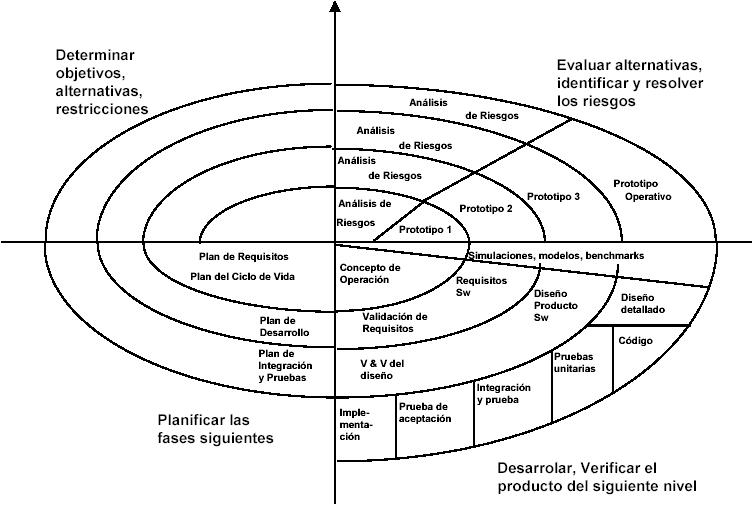
\includegraphics[width=16cm]{img/cap2/modelo_espiral}
  \end{center}
  \caption{Modelo en espiral.}
  \label{fig:modelo_espiral}
\end{figure}

Este modelo está dividido en ciclos. Cada ciclo representa una fase del proyecto y está dividido, a su vez, en 4 partes. Cada una de las partes tiene un objetivo distinto:

\begin{itemize}
\item \textbf{Determinar objetivos.} Se establecen las necesidades que debe cumplir el sistema en cada iteración teniendo en cuenta los objetivos finales. Según avanzan las iteraciones aumenta el coste del ciclo y su complejidad.
\item \textbf{Evaluar alternativas.} Se determinan diferentes formas de alcanzar los objetivos que se han establecido en la fase anterior. Se aborda el problema desde distintos puntos de vista, como, por ejemplo, el rendimiento del algoritmo en tiempo y espacio. Además, se consideran explícitamente los riesgos, intentando mitigarlos al máximo.
\item \textbf{Desarrollar y verificar.} Se desarrolla el producto siguiendo la mejor alternativa para poder alcanzar los objetivos del ciclo. Una vez diseñado e implementado el producto, se realizan las pruebas necesarias para comprobar su funcionamiento.
\item \textbf{Planificar.} Teniendo en cuenta los resultados de las pruebas realizadas, se planifica la siguiente iteración, se revisan los errores cometidos y se comienza un nuevo ciclo de la espiral.
\end{itemize}

\section{Plan de trabajo}
\label{sec:plandetrabajo}

Para poder abordar el problema se han marcado una serie de subobjetivos ha completar. Dichos hitos son los siguientes:

\begin{enumerate}
\item Estudio y comprensión de la composición de un mapa y como construirlo. Nos apoyaremos en las herramienta ofrecidas por ROS y que resultaran básicas para este fin, dicha herramientas son \textit{TF} \footnote{http://wiki.ros.org/tf} y \textit{Costmap}\footnotemark .
\footnotetext{http://wiki.ros.org/costmap\_2D}
\item Primer subobjetivo. Una vez conocido como funcionan los \textit{costmap} procederemos a crear un pequeño nodo en el que se cree un mapa con las observaciones instantáneas que percibimos con el láser.
\item Segundo subobjetivo. Extender el algoritmo anterior para poder añadir y eliminar objetos según entren o salgan de la escena.
\item Tercer subobjetivo. Modificar el paquete \textit{map\_server} para que acepte varios mapas como entrada y estudiar la manera de mezclar los mapas entre sí.
\item Fase de pruebas. Se le pasará al paquete de navegación de ROS, \textit{move\_base} ,el mapa resultante y se harán pruebas de navegación en el simulador y en el robot real.
\item Cuarto subobjetivo. Crear el mapa semántico, especificando las etiquetas naturales que tendrá una casa, salón, cocina, habitación... y usarlo para poder navegar a la estancia que le indiquemos.
\end{enumerate}
